\documentclass[twoside]{book}

% Packages required by doxygen
\usepackage{fixltx2e}
\usepackage{calc}
\usepackage{doxygen}
\usepackage[export]{adjustbox} % also loads graphicx
\usepackage{graphicx}
\usepackage[utf8]{inputenc}
\usepackage{makeidx}
\usepackage{multicol}
\usepackage{multirow}
\PassOptionsToPackage{warn}{textcomp}
\usepackage{textcomp}
\usepackage[nointegrals]{wasysym}
\usepackage[table]{xcolor}

% Font selection
\usepackage[T1]{fontenc}
\usepackage[scaled=.90]{helvet}
\usepackage{courier}
\usepackage{amssymb}
\usepackage{sectsty}
\renewcommand{\familydefault}{\sfdefault}
\allsectionsfont{%
  \fontseries{bc}\selectfont%
  \color{darkgray}%
}
\renewcommand{\DoxyLabelFont}{%
  \fontseries{bc}\selectfont%
  \color{darkgray}%
}
\newcommand{\+}{\discretionary{\mbox{\scriptsize$\hookleftarrow$}}{}{}}

% Page & text layout
\usepackage{geometry}
\geometry{%
  a4paper,%
  top=2.5cm,%
  bottom=2.5cm,%
  left=2.5cm,%
  right=2.5cm%
}
\tolerance=750
\hfuzz=15pt
\hbadness=750
\setlength{\emergencystretch}{15pt}
\setlength{\parindent}{0cm}
\setlength{\parskip}{3ex plus 2ex minus 2ex}
\makeatletter
\renewcommand{\paragraph}{%
  \@startsection{paragraph}{4}{0ex}{-1.0ex}{1.0ex}{%
    \normalfont\normalsize\bfseries\SS@parafont%
  }%
}
\renewcommand{\subparagraph}{%
  \@startsection{subparagraph}{5}{0ex}{-1.0ex}{1.0ex}{%
    \normalfont\normalsize\bfseries\SS@subparafont%
  }%
}
\makeatother

% Headers & footers
\usepackage{fancyhdr}
\pagestyle{fancyplain}
\fancyhead[LE]{\fancyplain{}{\bfseries\thepage}}
\fancyhead[CE]{\fancyplain{}{}}
\fancyhead[RE]{\fancyplain{}{\bfseries\leftmark}}
\fancyhead[LO]{\fancyplain{}{\bfseries\rightmark}}
\fancyhead[CO]{\fancyplain{}{}}
\fancyhead[RO]{\fancyplain{}{\bfseries\thepage}}
\fancyfoot[LE]{\fancyplain{}{}}
\fancyfoot[CE]{\fancyplain{}{}}
\fancyfoot[RE]{\fancyplain{}{\bfseries\scriptsize Generated by Doxygen }}
\fancyfoot[LO]{\fancyplain{}{\bfseries\scriptsize Generated by Doxygen }}
\fancyfoot[CO]{\fancyplain{}{}}
\fancyfoot[RO]{\fancyplain{}{}}
\renewcommand{\footrulewidth}{0.4pt}
\renewcommand{\chaptermark}[1]{%
  \markboth{#1}{}%
}
\renewcommand{\sectionmark}[1]{%
  \markright{\thesection\ #1}%
}

% Indices & bibliography
\usepackage{natbib}
\usepackage[titles]{tocloft}
\setcounter{tocdepth}{3}
\setcounter{secnumdepth}{5}
\makeindex

% Hyperlinks (required, but should be loaded last)
\usepackage{ifpdf}
\ifpdf
  \usepackage[pdftex,pagebackref=true]{hyperref}
\else
  \usepackage[ps2pdf,pagebackref=true]{hyperref}
\fi
\hypersetup{%
  colorlinks=true,%
  linkcolor=blue,%
  citecolor=blue,%
  unicode%
}

% Custom commands
\newcommand{\clearemptydoublepage}{%
  \newpage{\pagestyle{empty}\cleardoublepage}%
}

\usepackage{caption}
\captionsetup{labelsep=space,justification=centering,font={bf},singlelinecheck=off,skip=4pt,position=top}

%===== C O N T E N T S =====

\begin{document}

% Titlepage & ToC
\hypersetup{pageanchor=false,
             bookmarksnumbered=true,
             pdfencoding=unicode
            }
\pagenumbering{alph}
\begin{titlepage}
\vspace*{7cm}
\begin{center}%
{\Large Assignment1 }\\
\vspace*{1cm}
{\large Generated by Doxygen 1.8.13}\\
\end{center}
\end{titlepage}
\clearemptydoublepage
\pagenumbering{roman}
\tableofcontents
\clearemptydoublepage
\pagenumbering{arabic}
\hypersetup{pageanchor=true}

%--- Begin generated contents ---
\chapter{Hierarchical Index}
\section{Class Hierarchy}
This inheritance list is sorted roughly, but not completely, alphabetically\+:\begin{DoxyCompactList}
\item \contentsline{section}{ec.\+My\+Statistics}{\pageref{classec_1_1_my_statistics}}{}
\item \contentsline{section}{ec.\+Statistics}{\pageref{interfaceec_1_1_statistics}}{}
\begin{DoxyCompactList}
\item \contentsline{section}{ec.\+E\+C\+Statistics}{\pageref{classec_1_1_e_c_statistics}}{}
\end{DoxyCompactList}
\end{DoxyCompactList}

\chapter{Class Index}
\section{Class List}
Here are the classes, structs, unions and interfaces with brief descriptions\+:\begin{DoxyCompactList}
\item\contentsline{section}{\hyperlink{classec_1_1_e_c_statistics}{ec.\+E\+C\+Statistics} }{\pageref{classec_1_1_e_c_statistics}}{}
\item\contentsline{section}{\hyperlink{classec_1_1_my_statistics}{ec.\+My\+Statistics} }{\pageref{classec_1_1_my_statistics}}{}
\item\contentsline{section}{\hyperlink{interfaceec_1_1_statistics}{ec.\+Statistics} }{\pageref{interfaceec_1_1_statistics}}{}
\end{DoxyCompactList}

\chapter{Class Documentation}
\hypertarget{classec_1_1_e_c_statistics}{}\section{ec.\+E\+C\+Statistics Class Reference}
\label{classec_1_1_e_c_statistics}\index{ec.\+E\+C\+Statistics@{ec.\+E\+C\+Statistics}}
Inheritance diagram for ec.\+E\+C\+Statistics\+:\begin{figure}[H]
\begin{center}
\leavevmode
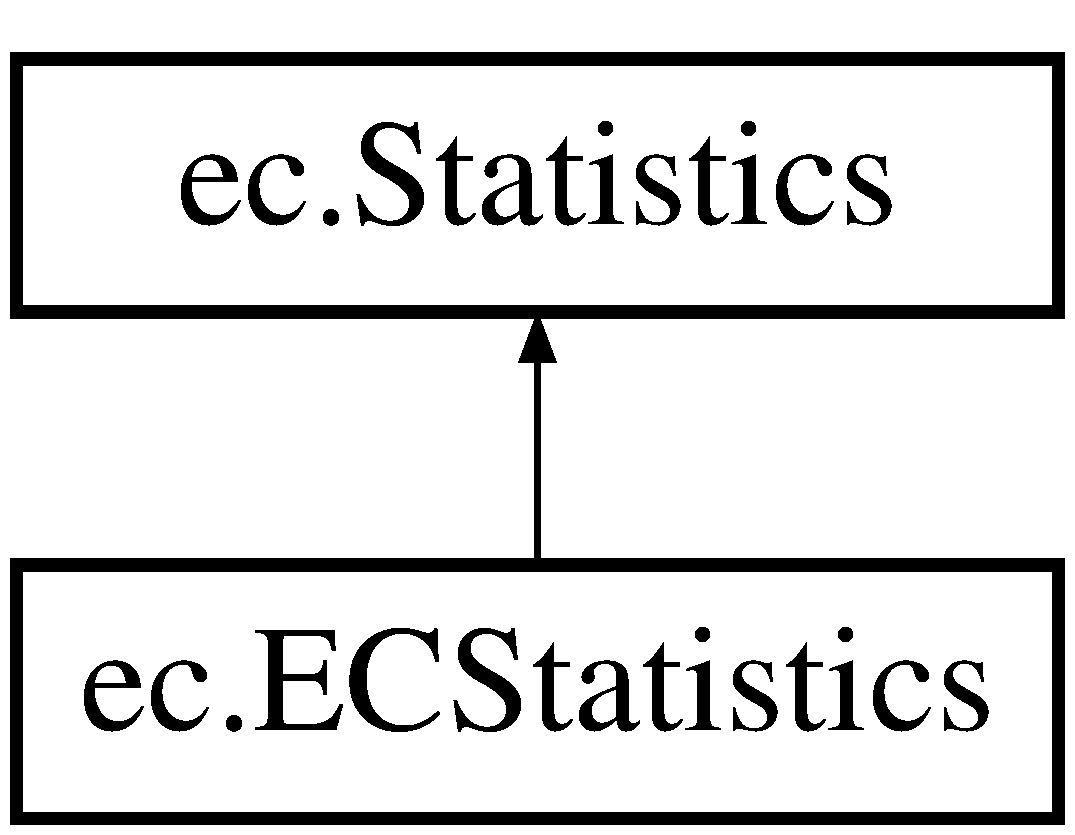
\includegraphics[height=2.000000cm]{classec_1_1_e_c_statistics}
\end{center}
\end{figure}
\subsection*{Public Member Functions}
\begin{DoxyCompactItemize}
\item 
void \hyperlink{classec_1_1_e_c_statistics_a60feff78d1b3a0b548544d9cfbd6a051}{add\+Data} (double value)
\begin{DoxyCompactList}\small\item\em Add data to statistics, which then calculates count, min, max, mean and stddev using incremental algorithms. \end{DoxyCompactList}\item 
double \hyperlink{classec_1_1_e_c_statistics_abb7e2fa1c13cea018e3cf1e2a82309db}{get\+Count} ()
\begin{DoxyCompactList}\small\item\em Retrieve count of data. \end{DoxyCompactList}\item 
double \hyperlink{classec_1_1_e_c_statistics_a2e37a5bd92ed681173461776f562375e}{get\+Min} ()
\begin{DoxyCompactList}\small\item\em Retrieve minimum value in data. \end{DoxyCompactList}\item 
double \hyperlink{classec_1_1_e_c_statistics_a5585b02f584a18bef7a792b76710c225}{get\+Max} ()
\begin{DoxyCompactList}\small\item\em Retrieve maximum value in data. \end{DoxyCompactList}\item 
double \hyperlink{classec_1_1_e_c_statistics_a62f3366afb939bb372e1ec1fd5aec3bc}{get\+Mean} ()
\begin{DoxyCompactList}\small\item\em Retrieve mean value in data. \end{DoxyCompactList}\item 
double \hyperlink{classec_1_1_e_c_statistics_a62cb7d1e5f86a179c68cc8a9c450b835}{get\+S\+TD} ()
\begin{DoxyCompactList}\small\item\em Retrieve standard deviation value in data. \end{DoxyCompactList}\item 
\mbox{\Hypertarget{classec_1_1_e_c_statistics_a120060ecbd8161d900c74f713ef3df22}\label{classec_1_1_e_c_statistics_a120060ecbd8161d900c74f713ef3df22}} 
void \hyperlink{classec_1_1_e_c_statistics_a120060ecbd8161d900c74f713ef3df22}{stats} ()
\begin{DoxyCompactList}\small\item\em Compute and update the data, to make sure it is more precise. \end{DoxyCompactList}\end{DoxyCompactItemize}


\subsection{Member Function Documentation}
\mbox{\Hypertarget{classec_1_1_e_c_statistics_a60feff78d1b3a0b548544d9cfbd6a051}\label{classec_1_1_e_c_statistics_a60feff78d1b3a0b548544d9cfbd6a051}} 
\index{ec\+::\+E\+C\+Statistics@{ec\+::\+E\+C\+Statistics}!add\+Data@{add\+Data}}
\index{add\+Data@{add\+Data}!ec\+::\+E\+C\+Statistics@{ec\+::\+E\+C\+Statistics}}
\subsubsection{\texorpdfstring{add\+Data()}{addData()}}
{\footnotesize\ttfamily void ec.\+E\+C\+Statistics.\+add\+Data (\begin{DoxyParamCaption}\item[{double}]{value }\end{DoxyParamCaption})}



Add data to statistics, which then calculates count, min, max, mean and stddev using incremental algorithms. 


\begin{DoxyParams}{Parameters}
{\em double} & value \\
\hline
\end{DoxyParams}


Implements \hyperlink{interfaceec_1_1_statistics_a8c59a234d776281dd7bd9fb05d0cb12e}{ec.\+Statistics}.

\mbox{\Hypertarget{classec_1_1_e_c_statistics_abb7e2fa1c13cea018e3cf1e2a82309db}\label{classec_1_1_e_c_statistics_abb7e2fa1c13cea018e3cf1e2a82309db}} 
\index{ec\+::\+E\+C\+Statistics@{ec\+::\+E\+C\+Statistics}!get\+Count@{get\+Count}}
\index{get\+Count@{get\+Count}!ec\+::\+E\+C\+Statistics@{ec\+::\+E\+C\+Statistics}}
\subsubsection{\texorpdfstring{get\+Count()}{getCount()}}
{\footnotesize\ttfamily double ec.\+E\+C\+Statistics.\+get\+Count (\begin{DoxyParamCaption}{ }\end{DoxyParamCaption})}



Retrieve count of data. 

\begin{DoxyReturn}{Returns}
double count 
\end{DoxyReturn}


Implements \hyperlink{interfaceec_1_1_statistics_aa9a82f2a37f7f6563106075872bc7af2}{ec.\+Statistics}.

\mbox{\Hypertarget{classec_1_1_e_c_statistics_a5585b02f584a18bef7a792b76710c225}\label{classec_1_1_e_c_statistics_a5585b02f584a18bef7a792b76710c225}} 
\index{ec\+::\+E\+C\+Statistics@{ec\+::\+E\+C\+Statistics}!get\+Max@{get\+Max}}
\index{get\+Max@{get\+Max}!ec\+::\+E\+C\+Statistics@{ec\+::\+E\+C\+Statistics}}
\subsubsection{\texorpdfstring{get\+Max()}{getMax()}}
{\footnotesize\ttfamily double ec.\+E\+C\+Statistics.\+get\+Max (\begin{DoxyParamCaption}{ }\end{DoxyParamCaption})}



Retrieve maximum value in data. 

\begin{DoxyReturn}{Returns}
double max 
\end{DoxyReturn}


Implements \hyperlink{interfaceec_1_1_statistics_a1cf8e3f12f56957e4133ce4cd07277dc}{ec.\+Statistics}.

\mbox{\Hypertarget{classec_1_1_e_c_statistics_a62f3366afb939bb372e1ec1fd5aec3bc}\label{classec_1_1_e_c_statistics_a62f3366afb939bb372e1ec1fd5aec3bc}} 
\index{ec\+::\+E\+C\+Statistics@{ec\+::\+E\+C\+Statistics}!get\+Mean@{get\+Mean}}
\index{get\+Mean@{get\+Mean}!ec\+::\+E\+C\+Statistics@{ec\+::\+E\+C\+Statistics}}
\subsubsection{\texorpdfstring{get\+Mean()}{getMean()}}
{\footnotesize\ttfamily double ec.\+E\+C\+Statistics.\+get\+Mean (\begin{DoxyParamCaption}{ }\end{DoxyParamCaption})}



Retrieve mean value in data. 

\begin{DoxyReturn}{Returns}
double mean 
\end{DoxyReturn}


Implements \hyperlink{interfaceec_1_1_statistics_aa25ad8afd473f6540041526226d946bd}{ec.\+Statistics}.

\mbox{\Hypertarget{classec_1_1_e_c_statistics_a2e37a5bd92ed681173461776f562375e}\label{classec_1_1_e_c_statistics_a2e37a5bd92ed681173461776f562375e}} 
\index{ec\+::\+E\+C\+Statistics@{ec\+::\+E\+C\+Statistics}!get\+Min@{get\+Min}}
\index{get\+Min@{get\+Min}!ec\+::\+E\+C\+Statistics@{ec\+::\+E\+C\+Statistics}}
\subsubsection{\texorpdfstring{get\+Min()}{getMin()}}
{\footnotesize\ttfamily double ec.\+E\+C\+Statistics.\+get\+Min (\begin{DoxyParamCaption}{ }\end{DoxyParamCaption})}



Retrieve minimum value in data. 

\begin{DoxyReturn}{Returns}
double min 
\end{DoxyReturn}


Implements \hyperlink{interfaceec_1_1_statistics_acee86eecccfe2d050c9a13a11f235d8d}{ec.\+Statistics}.

\mbox{\Hypertarget{classec_1_1_e_c_statistics_a62cb7d1e5f86a179c68cc8a9c450b835}\label{classec_1_1_e_c_statistics_a62cb7d1e5f86a179c68cc8a9c450b835}} 
\index{ec\+::\+E\+C\+Statistics@{ec\+::\+E\+C\+Statistics}!get\+S\+TD@{get\+S\+TD}}
\index{get\+S\+TD@{get\+S\+TD}!ec\+::\+E\+C\+Statistics@{ec\+::\+E\+C\+Statistics}}
\subsubsection{\texorpdfstring{get\+S\+T\+D()}{getSTD()}}
{\footnotesize\ttfamily double ec.\+E\+C\+Statistics.\+get\+S\+TD (\begin{DoxyParamCaption}{ }\end{DoxyParamCaption})}



Retrieve standard deviation value in data. 

\begin{DoxyReturn}{Returns}
double std 
\end{DoxyReturn}


Implements \hyperlink{interfaceec_1_1_statistics_a51643b39410b478bc996068eeb48ca0d}{ec.\+Statistics}.



The documentation for this class was generated from the following file\+:\begin{DoxyCompactItemize}
\item 
src/ec/E\+C\+Statistics.\+java\end{DoxyCompactItemize}

\hypertarget{classec_1_1_my_statistics}{}\section{ec.\+My\+Statistics Class Reference}
\label{classec_1_1_my_statistics}\index{ec.\+My\+Statistics@{ec.\+My\+Statistics}}
\subsection*{Static Public Member Functions}
\begin{DoxyCompactItemize}
\item 
\mbox{\Hypertarget{classec_1_1_my_statistics_a94ebe0fcc6975203107c041bb71b0880}\label{classec_1_1_my_statistics_a94ebe0fcc6975203107c041bb71b0880}} 
static void {\bfseries main} (String\mbox{[}$\,$\mbox{]} args)
\end{DoxyCompactItemize}


The documentation for this class was generated from the following file\+:\begin{DoxyCompactItemize}
\item 
src/ec/My\+Statistics.\+java\end{DoxyCompactItemize}

\hypertarget{interfaceec_1_1_statistics}{}\section{ec.\+Statistics Interface Reference}
\label{interfaceec_1_1_statistics}\index{ec.\+Statistics@{ec.\+Statistics}}
Inheritance diagram for ec.\+Statistics\+:\begin{figure}[H]
\begin{center}
\leavevmode
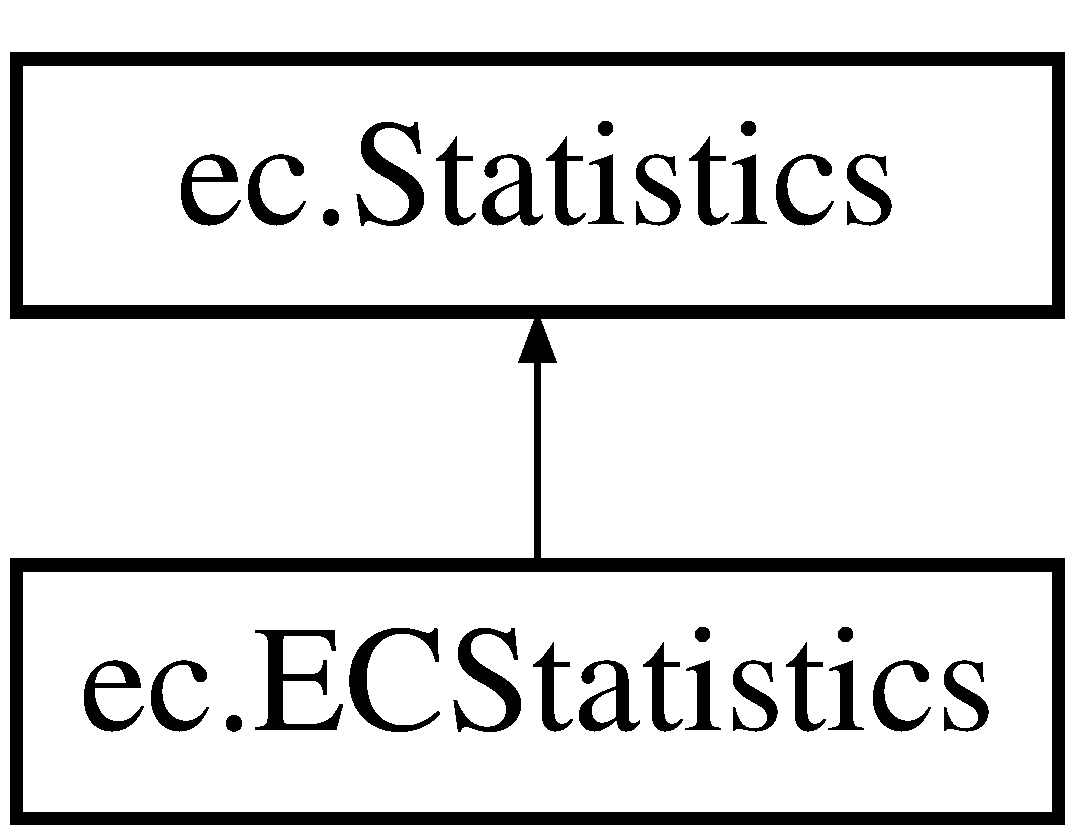
\includegraphics[height=2.000000cm]{interfaceec_1_1_statistics}
\end{center}
\end{figure}
\subsection*{Public Member Functions}
\begin{DoxyCompactItemize}
\item 
void \hyperlink{interfaceec_1_1_statistics_a8c59a234d776281dd7bd9fb05d0cb12e}{add\+Data} (double value)
\begin{DoxyCompactList}\small\item\em Add data to statistics, which then calculates count, min, max, mean and stddev using incremental algorithms. \end{DoxyCompactList}\item 
double \hyperlink{interfaceec_1_1_statistics_aa9a82f2a37f7f6563106075872bc7af2}{get\+Count} ()
\begin{DoxyCompactList}\small\item\em Retrieve count of data. \end{DoxyCompactList}\item 
double \hyperlink{interfaceec_1_1_statistics_acee86eecccfe2d050c9a13a11f235d8d}{get\+Min} ()
\begin{DoxyCompactList}\small\item\em Retrieve minimum value in data. \end{DoxyCompactList}\item 
double \hyperlink{interfaceec_1_1_statistics_a1cf8e3f12f56957e4133ce4cd07277dc}{get\+Max} ()
\begin{DoxyCompactList}\small\item\em Retrieve maximum value in data. \end{DoxyCompactList}\item 
double \hyperlink{interfaceec_1_1_statistics_aa25ad8afd473f6540041526226d946bd}{get\+Mean} ()
\begin{DoxyCompactList}\small\item\em Retrieve mean value in data. \end{DoxyCompactList}\item 
double \hyperlink{interfaceec_1_1_statistics_a51643b39410b478bc996068eeb48ca0d}{get\+S\+TD} ()
\begin{DoxyCompactList}\small\item\em Retrieve standard deviation value in data. \end{DoxyCompactList}\item 
\mbox{\Hypertarget{interfaceec_1_1_statistics_a648ce66b63ce750a16af8398c1ea4d8b}\label{interfaceec_1_1_statistics_a648ce66b63ce750a16af8398c1ea4d8b}} 
void \hyperlink{interfaceec_1_1_statistics_a648ce66b63ce750a16af8398c1ea4d8b}{stats} ()
\begin{DoxyCompactList}\small\item\em Compute and update the data, to make sure it is more precise. \end{DoxyCompactList}\end{DoxyCompactItemize}


\subsection{Member Function Documentation}
\mbox{\Hypertarget{interfaceec_1_1_statistics_a8c59a234d776281dd7bd9fb05d0cb12e}\label{interfaceec_1_1_statistics_a8c59a234d776281dd7bd9fb05d0cb12e}} 
\index{ec\+::\+Statistics@{ec\+::\+Statistics}!add\+Data@{add\+Data}}
\index{add\+Data@{add\+Data}!ec\+::\+Statistics@{ec\+::\+Statistics}}
\subsubsection{\texorpdfstring{add\+Data()}{addData()}}
{\footnotesize\ttfamily void ec.\+Statistics.\+add\+Data (\begin{DoxyParamCaption}\item[{double}]{value }\end{DoxyParamCaption})}



Add data to statistics, which then calculates count, min, max, mean and stddev using incremental algorithms. 


\begin{DoxyParams}{Parameters}
{\em double} & value \\
\hline
\end{DoxyParams}


Implemented in \hyperlink{classec_1_1_e_c_statistics_a60feff78d1b3a0b548544d9cfbd6a051}{ec.\+E\+C\+Statistics}.

\mbox{\Hypertarget{interfaceec_1_1_statistics_aa9a82f2a37f7f6563106075872bc7af2}\label{interfaceec_1_1_statistics_aa9a82f2a37f7f6563106075872bc7af2}} 
\index{ec\+::\+Statistics@{ec\+::\+Statistics}!get\+Count@{get\+Count}}
\index{get\+Count@{get\+Count}!ec\+::\+Statistics@{ec\+::\+Statistics}}
\subsubsection{\texorpdfstring{get\+Count()}{getCount()}}
{\footnotesize\ttfamily double ec.\+Statistics.\+get\+Count (\begin{DoxyParamCaption}{ }\end{DoxyParamCaption})}



Retrieve count of data. 

\begin{DoxyReturn}{Returns}
double count 
\end{DoxyReturn}


Implemented in \hyperlink{classec_1_1_e_c_statistics_abb7e2fa1c13cea018e3cf1e2a82309db}{ec.\+E\+C\+Statistics}.

\mbox{\Hypertarget{interfaceec_1_1_statistics_a1cf8e3f12f56957e4133ce4cd07277dc}\label{interfaceec_1_1_statistics_a1cf8e3f12f56957e4133ce4cd07277dc}} 
\index{ec\+::\+Statistics@{ec\+::\+Statistics}!get\+Max@{get\+Max}}
\index{get\+Max@{get\+Max}!ec\+::\+Statistics@{ec\+::\+Statistics}}
\subsubsection{\texorpdfstring{get\+Max()}{getMax()}}
{\footnotesize\ttfamily double ec.\+Statistics.\+get\+Max (\begin{DoxyParamCaption}{ }\end{DoxyParamCaption})}



Retrieve maximum value in data. 

\begin{DoxyReturn}{Returns}
double max 
\end{DoxyReturn}


Implemented in \hyperlink{classec_1_1_e_c_statistics_a5585b02f584a18bef7a792b76710c225}{ec.\+E\+C\+Statistics}.

\mbox{\Hypertarget{interfaceec_1_1_statistics_aa25ad8afd473f6540041526226d946bd}\label{interfaceec_1_1_statistics_aa25ad8afd473f6540041526226d946bd}} 
\index{ec\+::\+Statistics@{ec\+::\+Statistics}!get\+Mean@{get\+Mean}}
\index{get\+Mean@{get\+Mean}!ec\+::\+Statistics@{ec\+::\+Statistics}}
\subsubsection{\texorpdfstring{get\+Mean()}{getMean()}}
{\footnotesize\ttfamily double ec.\+Statistics.\+get\+Mean (\begin{DoxyParamCaption}{ }\end{DoxyParamCaption})}



Retrieve mean value in data. 

\begin{DoxyReturn}{Returns}
double mean 
\end{DoxyReturn}


Implemented in \hyperlink{classec_1_1_e_c_statistics_a62f3366afb939bb372e1ec1fd5aec3bc}{ec.\+E\+C\+Statistics}.

\mbox{\Hypertarget{interfaceec_1_1_statistics_acee86eecccfe2d050c9a13a11f235d8d}\label{interfaceec_1_1_statistics_acee86eecccfe2d050c9a13a11f235d8d}} 
\index{ec\+::\+Statistics@{ec\+::\+Statistics}!get\+Min@{get\+Min}}
\index{get\+Min@{get\+Min}!ec\+::\+Statistics@{ec\+::\+Statistics}}
\subsubsection{\texorpdfstring{get\+Min()}{getMin()}}
{\footnotesize\ttfamily double ec.\+Statistics.\+get\+Min (\begin{DoxyParamCaption}{ }\end{DoxyParamCaption})}



Retrieve minimum value in data. 

\begin{DoxyReturn}{Returns}
double min 
\end{DoxyReturn}


Implemented in \hyperlink{classec_1_1_e_c_statistics_a2e37a5bd92ed681173461776f562375e}{ec.\+E\+C\+Statistics}.

\mbox{\Hypertarget{interfaceec_1_1_statistics_a51643b39410b478bc996068eeb48ca0d}\label{interfaceec_1_1_statistics_a51643b39410b478bc996068eeb48ca0d}} 
\index{ec\+::\+Statistics@{ec\+::\+Statistics}!get\+S\+TD@{get\+S\+TD}}
\index{get\+S\+TD@{get\+S\+TD}!ec\+::\+Statistics@{ec\+::\+Statistics}}
\subsubsection{\texorpdfstring{get\+S\+T\+D()}{getSTD()}}
{\footnotesize\ttfamily double ec.\+Statistics.\+get\+S\+TD (\begin{DoxyParamCaption}{ }\end{DoxyParamCaption})}



Retrieve standard deviation value in data. 

\begin{DoxyReturn}{Returns}
double std 
\end{DoxyReturn}


Implemented in \hyperlink{classec_1_1_e_c_statistics_a62cb7d1e5f86a179c68cc8a9c450b835}{ec.\+E\+C\+Statistics}.



The documentation for this interface was generated from the following file\+:\begin{DoxyCompactItemize}
\item 
src/ec/Statistics.\+java\end{DoxyCompactItemize}

%--- End generated contents ---

% Index
\backmatter
\newpage
\phantomsection
\clearemptydoublepage
\addcontentsline{toc}{chapter}{Index}
\printindex

\end{document}
